\documentclass{beamer}
\usepackage[utf8]{inputenc}
\usepackage{graphicx, epsfig}
\usepackage{amsmath,mathrsfs,amsfonts,amssymb}
\usepackage{floatflt}
\usepackage{epic,ecltree}
\usepackage{mathtext}
\usepackage{fancybox}
\usepackage{fancyhdr}
\usepackage{multirow}
\usepackage{enumerate}
\usepackage{epstopdf}
\usepackage{multicol}
\usepackage{algorithm}
\usepackage[noend]{algorithmic}
\usepackage{tikz}
\usepackage{blindtext}
\usetheme{default}%{Singapore}%{Warsaw}%{Warsaw}%{Darmstadt}
\usecolortheme{default}

\setbeamerfont{title}{size=\Huge}
\setbeamertemplate{footline}[page number]{}

\setbeamertemplate{section in toc}[sections numbered]


\makeatletter
\newcommand\HUGE{\@setfontsize\Huge{35}{40}}
\makeatother    

\setbeamerfont{title}{size=\HUGE}
\beamertemplatenavigationsymbolsempty

% latin bold lower
\newcommand{\ba}{\mathbf{a}} 
\newcommand{\bc}{\mathbf{c}} 
\newcommand{\be}{\mathbf{e}} 
\newcommand{\bh}{\mathbf{h}} 
\newcommand{\bp}{\mathbf{p}} 
\newcommand{\bt}{\mathbf{t}} 
\newcommand{\bs}{\mathbf{s}} 
\newcommand{\bu}{\mathbf{u}} 
\newcommand{\bv}{\mathbf{v}} 
\newcommand{\bw}{\mathbf{w}} 
\newcommand{\bx}{\mathbf{x}} 
\newcommand{\by}{\mathbf{y}} 
\newcommand{\bz}{\mathbf{z}} 

% latin bold upper
\newcommand{\bA}{\mathbf{A}} 
\newcommand{\bB}{\mathbf{B}} 
\newcommand{\bC}{\mathbf{C}} 
\newcommand{\bI}{\mathbf{I}} 
\newcommand{\bL}{\mathbf{L}} 
\newcommand{\bM}{\mathbf{M}} 
\newcommand{\bQ}{\mathbf{Q}} 
\newcommand{\bT}{\mathbf{T}} 
\newcommand{\bU}{\mathbf{U}} 
\newcommand{\bV}{\mathbf{V}} 
\newcommand{\bW}{\mathbf{W}} 
\newcommand{\bX}{\mathbf{X}} 
\newcommand{\bY}{\mathbf{Y}} 
\newcommand{\bZ}{\mathbf{Z}} 

% latin cal upper
\newcommand{\cG}{\mathcal{G}} 
\newcommand{\cL}{\mathcal{L}} 
\newcommand{\cN}{\mathcal{N}} 
\newcommand{\cS}{\mathcal{S}} 
\newcommand{\cT}{\mathcal{T}} 
\newcommand{\cW}{\mathcal{W}} 
\newcommand{\cX}{\mathcal{X}} 
\newcommand{\cZ}{\mathcal{Z}} 

% latin bb upper
\newcommand{\bbE}{\mathbb{E}} 
\newcommand{\bbI}{\mathbb{I}} 
\newcommand{\bbP}{\mathbb{P}} 
\newcommand{\bbR}{\mathbb{R}} 

% greek bold lower
\newcommand{\bepsilon}{\boldsymbol{\epsilon}} 
\newcommand{\btheta}{\boldsymbol{\theta}} 
\newcommand{\blambda}{\boldsymbol{\lambda}} 
\newcommand{\bpi}{\boldsymbol{\pi}} 
\newcommand{\bmu}{\boldsymbol{\mu}} 
\newcommand{\bsigma}{\boldsymbol{\sigma}} 
\newcommand{\bphi}{\boldsymbol{\phi}} 

% greek bold upper
\newcommand{\bSigma}{\boldsymbol{\Sigma}} 

\DeclareMathOperator*{\argmin}{arg\,min}
\DeclareMathOperator*{\argmax}{arg\,max}

\newcommand{\createdgmtitle}[1]{\title[\hbox to 56mm{Deep Generative Models  \hfill\insertframenumber\,/\,\inserttotalframenumber}]
	{Deep Generative Models \\ {\Huge Lecture #1}}
	\author{Roman Isachenko}
	\institute{
\includegraphics[width=0.5cm]{../utils/ozonmasterslogo} \large{Ozon Masters}}
	\date{Spring, 2022}
}

\newcommand\myfootnote[1]{%
  \tikz[remember picture,overlay]
  \draw (current page.south west) +(1in + \oddsidemargin,0.5em)
  node[anchor=south west,inner sep=0pt]{\parbox{\textwidth}{%
      \rlap{\rule{10em}{0.4pt}}\raggedright\scriptsize \textit{#1}}};}

\newcommand\myfootnotewithlink[2]{%
  \tikz[remember picture,overlay]
  \draw (current page.south west) +(1in + \oddsidemargin,0.5em)
  node[anchor=south west,inner sep=0pt]{\parbox{\textwidth}{%
      \rlap{\rule{10em}{0.4pt}}\raggedright\scriptsize\href{#1}{\textit{#2}}}};}
      
\AtBeginSection[]
{
	\begin{frame}{Outline}
		\tableofcontents[currentsection,subsectionstyle=hide]
	\end{frame}
}
\AtBeginSubsection[]{
	\begin{frame}{Outline}
		\tableofcontents[currentsection,currentsubsection]
	\end{frame}
}
\createdgmtitle{3}
%--------------------------------------------------------------------------------
\begin{document}
%--------------------------------------------------------------------------------
\begin{frame}[noframenumbering,plain]
%\thispagestyle{empty}
\titlepage
\end{frame}
%=======
\begin{frame}{Recap of previous lecture}
	\begin{block}{MLE problem for autoregressive model}
		\vspace{-0.7cm}
		\[
		\btheta^* = \argmax_{\btheta} p(\bX | \btheta) = \argmax_{\btheta} \sum_{i=1}^n \sum_{j=1}^m \log p(x_{ij} | \bx_{i, 1:j - 1}\btheta).
		\]
		\vspace{-0.7cm}
	\end{block}
	\begin{block}{Sampling}
		\vspace{-0.5cm}
		\[
			\hat{x}_1 \sim p(x_1 | \btheta), \quad \hat{x}_2 \sim p(x_2 | \hat{x}_1, \btheta), \dots, \quad \hat{x}_m \sim p(x_m | \hat{\bx}_{1:m-1}, \btheta)
		\]
		New generated object is $\hat{\bx} = (\hat{x}_1, \hat{x}_2, \dots, \hat{x}_m)$.
	\end{block}
	Masking helps to make neural network autoregressive.
	\begin{itemize}
		\item \textbf{MADE} - masked autoencoder (MLP).
		\item \textbf{WaveNet} - masked 1D convolutions.
		\item \textbf{PixelCNN} - masked 2D convolutions.
	\end{itemize}
	\textbf{PixelCNN++} uses discretized mixture of logistic distribution to make the output distribution more natural.
\end{frame}
%=======
\begin{frame}{Recap of previous lecture}
	\begin{block}{Posterior distribution}
		\[
		p(\btheta | \bX) = \frac{p(\bX | \btheta) p(\btheta)}{p(\bX)} = \frac{p(\bX | \btheta) p(\btheta)}{\int p(\bX | \btheta) p(\btheta) d \btheta} 
		\]
		\vspace{-0.2cm}
	\end{block}
	\begin{block}{Bayesian inference}
		\vspace{-0.2cm}
		\[
		p(\bx | \bX) = \int p(\bx | \btheta) p(\btheta | \bX) d \btheta
		\]
		\vspace{-0.2cm}
	\end{block}
	\begin{block}{Maximum a posteriori (MAP) estimation}
		\vspace{-0.2cm}
		\[
		\btheta^* = \argmax_{\btheta} p(\btheta | \bX) = \argmax_{\btheta} \bigl(\log p(\bX | \btheta) + \log p(\btheta) \bigr)
		\]
		\vspace{-0.2cm}
	\end{block}
	\begin{block}{MAP inference}
		\[
		p(\bx | \bX) = \int p(\bx| \btheta) p(\btheta | \bX ) d \btheta \approx p(\bx | \btheta^*).
		\]
	\end{block}
\end{frame}
%=======
\begin{frame}{Variational lower bound (ELBO)}
	\begin{block}{Derivation 1}
		\vspace{-0.7cm}
		\begin{multline*}
			\log p(\bx| \btheta) 
			= \log \int p(\bx, \bz | \btheta) d\bz = \\ 
			= \log \int \frac{q(\bz)}{q(\bz)} p(\bx, \bz | \btheta) d\bz
			= \log \bbE_{q} \left[\frac{p(\bx, \bz| \btheta)}{q(\bz)} \right] \geq \\
			\geq \bbE_{q} \log \frac{p(\bx, \bz| \btheta)}{q(\bz)} = \int q(\bz) \log \frac{p(\bx, \bz| \btheta)}{q(\bz)} d \bz = \cL(q, \btheta)
		\end{multline*}
		\vspace{-0.7cm}
	\end{block}
	\begin{block}{Derivation 2}
		\vspace{-0.7cm}
		\begin{multline*}
			\log p(\bx| \btheta) 
			= \int q(\bz) \log p(\bx| \btheta) d\bz = \\ 
			= \int q(\bz) \log \frac{p(\bx, \bz| \btheta)}{p(\bz|\bx, \btheta)}d\bz
			= \int q(\bz) \log \frac{p(\bx, \bz| \btheta) q(\bz)}{p(\bz|\bx, \btheta) q(\bz)} d\bz = \\
			= \int q(\bz) \log \frac{p(\bx, \bz | \btheta)}{q(\bz)}d\bz + \int q(\bz) \log \frac{q(\bz)}{p(\bz|\bx, \btheta)}d\bz = \\ 
			= \mathcal{L} (q, \btheta) + KL(q(\bz) || p(\bz|\bx, \btheta)) \geq \mathcal{L} (q, \btheta).
		\end{multline*}
		\vspace{-0.7cm}
	\end{block}
\end{frame}
%=======
\begin{frame}{Variational lower bound}
	\vspace{-0.5cm}
	\begin{align*}
 	 \mathcal{L} (q, \btheta) &= \int q(\bz) \log \frac{p(\bx, \bz | \btheta)}{q(\bz)}d\bz = \\ 
	  &= \int q(\bz) \log p(\bx | \bz, \btheta) d\bz + \int q(\bz) \log \frac{p(\bz)}{q(\bz)}d\bz \\ 
	  &= \mathbb{E}_{q} \log p(\bx | \bz, \btheta) - KL (q(\bz) || p(\bz))
	\end{align*}
	\vspace{-0.5cm}
	\begin{block}{Log-likelihood decomposition}
		\vspace{-0.5cm}
		\[
			 \log p(\bx| \btheta) = \mathbb{E}_{q} \log p(\bx | \bz, \btheta) - KL (q(\bz) || p(\bz)) + KL(q(\bz) || p(\bz|\bx, \btheta)).
		\]
	\end{block}
	\begin{itemize}
	\item Instead of maximizing incomplete likelihood, maximize ELBO
   	\[
	    \max_{\btheta} p(\bx | \btheta) \quad \rightarrow \quad \max_{q, \btheta} \mathcal{L} (q, \btheta)
   	\]
   	\item Maximization of ELBO by variational distribution $q$ is equivalent to minimization of KL
  	\[
	    \max_q \mathcal{L} (q, \btheta) \equiv \min_q KL(q(\bz) || p(\bz|\bx, \btheta)).
  	\]
  	\end{itemize}
	   	    
\end{frame}
%=======
\begin{frame}{EM-algorithm}
	\[
		\mathcal{L} (q, \btheta)  = \int q(\bz) \log p(\bx | \bz, \btheta) d\bz + \int q(\bz) \log \frac{p(\bz)}{q(\bz)}d\bz.
	\]
	\begin{block}{Block-coordinate optimization}
	\begin{itemize}
		\item Initialize $\btheta^*$;
		\item E-step
		\begin{multline*}
			q^*(\bz) = \argmax_q \mathcal{L} (q, \btheta^*) = \\
			= \argmin_q KL(q(\bz) || p(\bz | \bx, \btheta^*)) = p(\bz| \bx, \btheta^*);
		\end{multline*}
		\item M-step
		\[
			\btheta^* = \argmax_{\btheta} \mathcal{L} (q^*, \btheta);
		\]
		\item Repeat E-step and M-step until convergence.
	\end{itemize}
	\end{block}
\end{frame}
%=======
\begin{frame}{EM illustration}
	
	\begin{minipage}[t]{0.45\columnwidth}
		\begin{figure}
			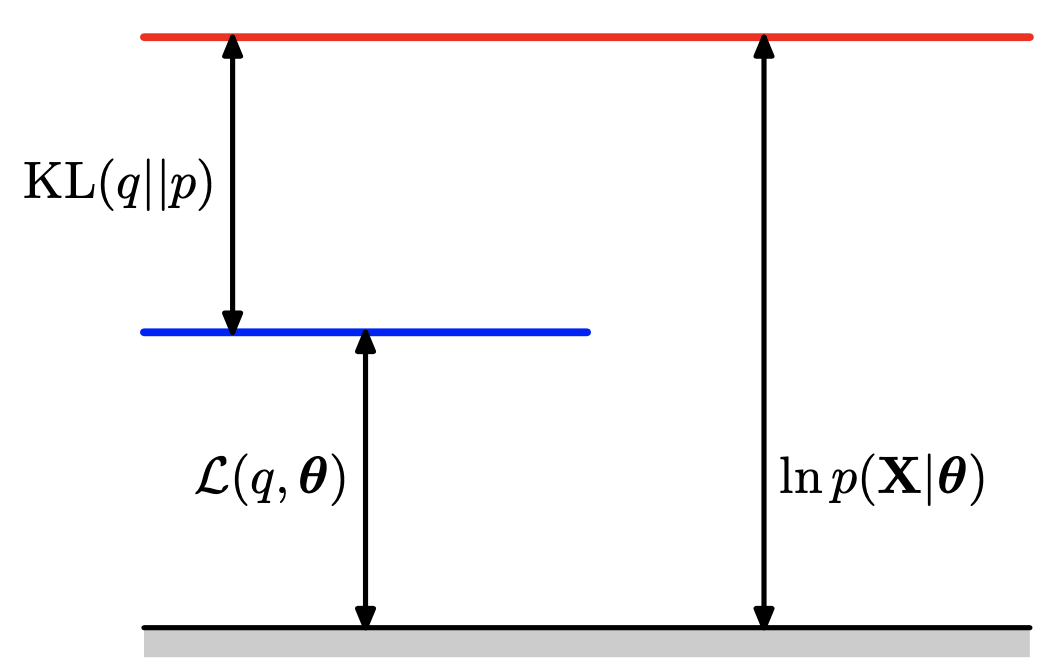
\includegraphics[width=0.9\linewidth]{figs/em_bishop1}
		\end{figure}
	\end{minipage}%
	\begin{minipage}[t]{0.55\columnwidth}
		\begin{figure}
			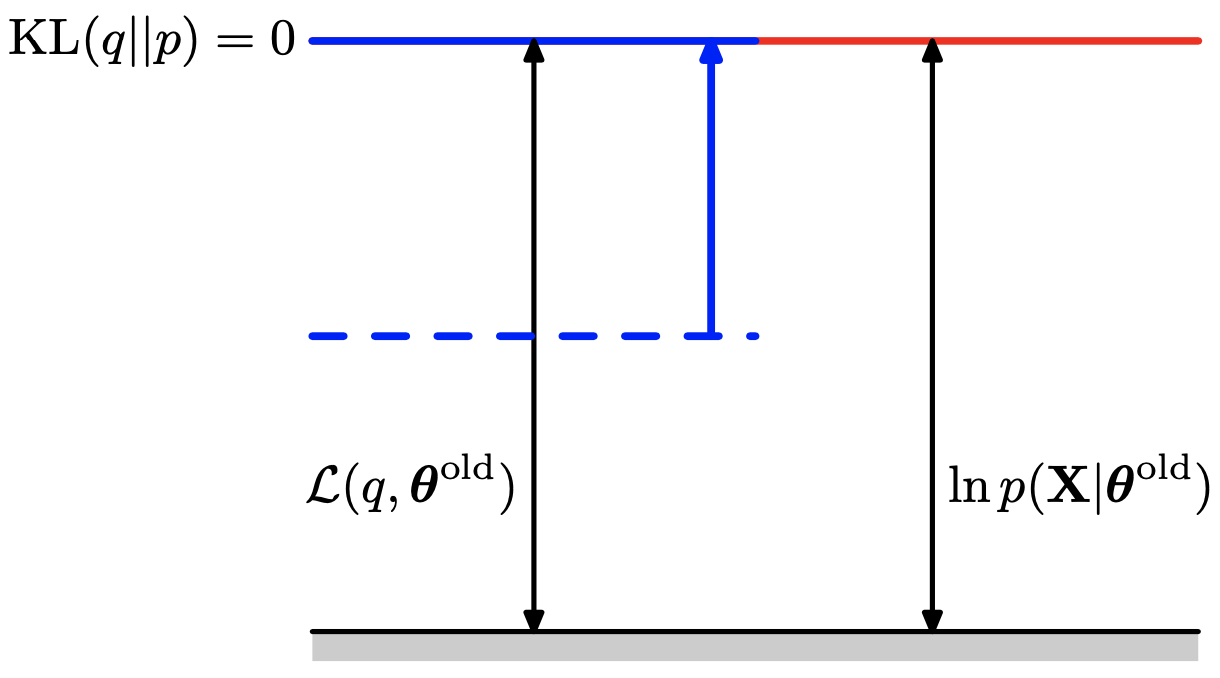
\includegraphics[width=0.85\linewidth]{figs/em_bishop2}
		\end{figure}
	\end{minipage}
	\begin{figure}
		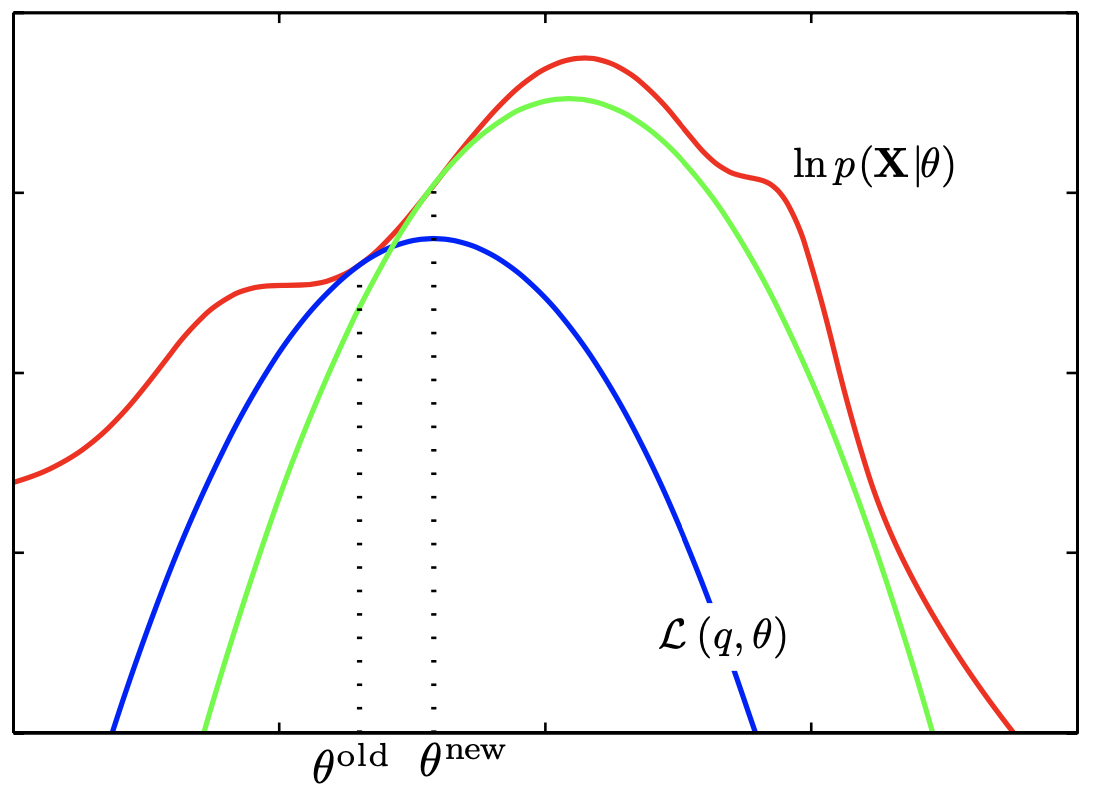
\includegraphics[width=.55\linewidth]{figs/em_bishop3}
	\end{figure}

	\myfootnote{Bishop\,C. Pattern Recognition and Machine Learning, 2006}
\end{frame}
%=======
\begin{frame}{Amortized variational inference}
    \begin{block}{E-step}
    \vspace{-0.3cm}
    \[
		q(\bz) = \argmax_q \mathcal{L} (q, \btheta^*) = \argmin_q KL(q || p) =
		 p(\bz| \bx, \btheta^*).
	\]
	\begin{itemize}
		\item $p(\bz| \bx, \btheta^*)$ could be \textbf{intractable};
		\item $q(\bz)$ is different for each object $\bx$.
	\end{itemize}
    \end{block}
	\begin{block}{Idea}
	Restrict a family of all possible distributions $q(\bz)$ to a parametric class $q(\bz|\bx, \bphi)$ conditioned on samples $\bx$ with parameters $\bphi$.
	\end{block}
	
	\textbf{Variational Bayes}
	\begin{itemize}
		\item E-step
		\[
		\bphi_k = \bphi_{k-1} + \left.\eta \nabla_{\bphi} \mathcal{L}(\bphi, \btheta_{k-1})\right|_{\bphi=\bphi_{k-1}}
		\]
		\item M-step
		\[
		\btheta_k = \btheta_{k-1} + \left.\eta \nabla_{\btheta} \mathcal{L}(\bphi_k, \btheta)\right|_{\btheta=\btheta_{k-1}}
		\]
	\end{itemize}
\end{frame}
%=======
\begin{frame}{Variational EM-algorithm}
	\begin{block}{ELBO}
		\vspace{-0.5cm}
		\[
			\log p(\bx| \btheta) = \mathcal{L} (\bphi, \btheta) + KL(q(\bz | \bx, \bphi) || p(\bz|\bx, \btheta)) \geq \mathcal{L} (\bphi, \btheta).
		\]
		\vspace{-0.5cm}
	\end{block}
	\begin{itemize}
		\item E-step
		\[
		\bphi_k = \bphi_{k-1} + \left.\eta \nabla_{\bphi} \mathcal{L}(\bphi, \btheta_{k-1})\right|_{\bphi=\bphi_{k-1}},
		\]
		where $\bphi$~-- parameters of variational distribution $q(\bz | \bx, \bphi)$.
		\item M-step
		\[
		\btheta_k = \btheta_{k-1} + \left.\eta \nabla_{\btheta} \mathcal{L}(\bphi_k, \btheta)\right|_{\btheta=\btheta_{k-1}},
		\]
		where $\btheta$~-- parameters of the generative distribution $p(\bx | \bz, \btheta)$.
	\end{itemize}
	Now all we have to do is to obtain two gradients $\nabla_{\bphi} \mathcal{L}(\bphi, \btheta)$, $\nabla_{\btheta} \mathcal{L}(\bphi, \btheta)$.  \\
	\textbf{Challenge:} Number of samples $n$ could be huge (we heed to derive unbiased stochastic gradients).
\end{frame}
%=======
\begin{frame}{ELBO gradients}
	\[
		 \mathcal{L} (\bphi, \btheta)  = \mathbb{E}_{q} \left[\log p(\bx | \bz, \btheta) + \log \frac{p(\bz)}{q(\bz | \bx, \bphi)} \right] \rightarrow \max_{\bphi, \btheta}.
	\]	
	\begin{block}{M-step: $\nabla_{\btheta} \mathcal{L}(\bphi, \btheta)$}
		\vspace{-0.7cm}
		\begin{multline*}
			\nabla_{\btheta} \mathcal{L} (\bphi, \btheta)
			= \int q(\bz|\bx, \bphi) \nabla_{\btheta}\log p(\bx|\bz, \btheta) d \bz \approx  \\
			\approx \nabla_{\btheta}\log p(\bx|\bz^*, \btheta), \quad \bz^* \sim q(\bz|\bx, \bphi).
		\end{multline*}
		\vspace{-0.7cm}
	\end{block}
	\begin{block}{E-step: $\nabla_{\bphi} \mathcal{L}(\bphi, \btheta)$}
	Difference from M-step: density function $q(\bz| \bx, \bphi)$ depends on the parameters $\bphi$, it is impossible to use the Monte-Carlo estimation:
	\begin{align*}
		\nabla_{\bphi} \mathcal{L} (\bphi, \btheta) &= \nabla_{\bphi} \int q(\bz | \bx, \bphi) \left[\log p(\bx | \bz, \btheta) + \log \frac{p(\bz)}{q(\bz| \bx, \bphi)} \right] d \bz \\
		& \neq  \int q(\bz | \bx, \bphi) \nabla_{\bphi} \left[\log p(\bx | \bz, \btheta) + \log \frac{p(\bz)}{q(\bz| \bx, \bphi)} \right] d \bz \\
	\end{align*}
	\end{block}
\end{frame}
%=======
\begin{frame}{Summary}
	\begin{itemize}
		\item LVM maximizes variational evidence lower bound (ELBO) to find MLE of model parameters.
		\vfill
		\item The general variational EM algorithm maximizes ELBO objective.
		\vfill
		\item Amortized inference allows to efficiently compute stochastic gradients for ELBO using Monte-Carlo estimation.
	\end{itemize}
\end{frame}
%=======
\end{document} 